\documentclass[tikz,svgnames]{standalone}

\usepackage{mathtools}

\usetikzlibrary{calc}

\renewcommand\vec[1]{\boldsymbol{#1}}

\begin{document}
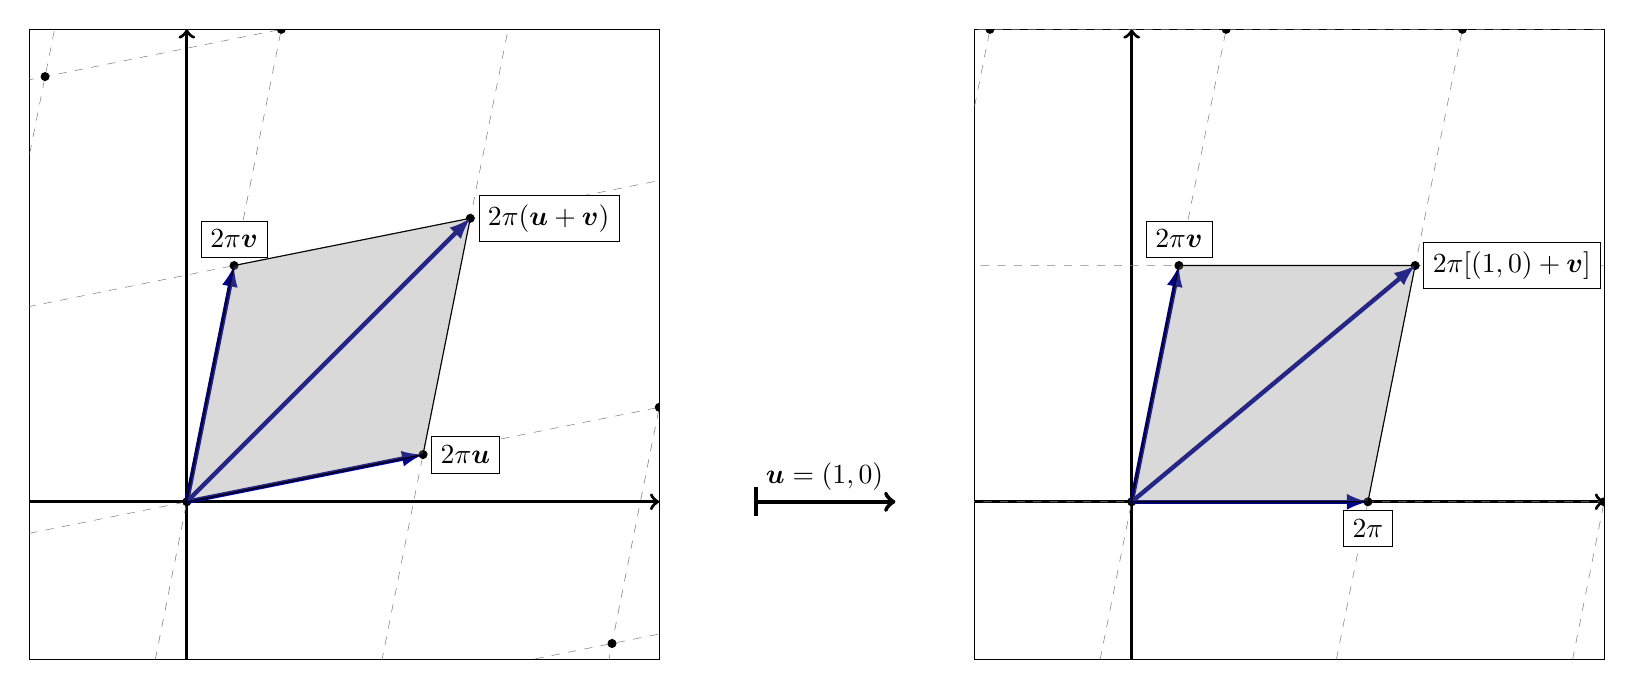
\begin{tikzpicture}[
    label/.style={black,draw,fill=white,ultra thin},
    vector/.style={ultra thick,-latex,DarkBlue}
  ]

  \def\xmin{-2} \def\xmax{6}
  \def\ymin{-2} \def\ymax{6}
  \def\gridscale{3}

  \begin{scope}
    \coordinate (origin) at (0,0);

    \draw [very thick,->] (\xmin,0) -- (\xmax,0);
    \draw [very thick,->] (0,\ymin) -- (0,\ymax);
    \clip [draw] (\xmin,\ymin) rectangle (\xmax,\ymax);

    \pgftransformcm{1}{0.2}{0.2}{1}{\pgfpoint{0}{0}}

    \draw[style=help lines,dashed] (\xmin-\xmax,\ymin-\ymax) grid[step=\gridscale] (-\xmin+\xmax,-\ymin+\ymax);

    \foreach \x in {\xmin,...,\xmax}{
        \foreach \y in {\ymin,...,\ymax}{
            \node[draw,circle,inner sep=1pt,fill] at (\gridscale*\x,\gridscale*\y) {};
          }
      }

    \draw [vector] (origin) -- (\gridscale,0) node [label,right=3] {$2 \pi \vec u$};
    \draw [vector] (origin) -- (0,\gridscale) node [label,above=3] {$2 \pi \vec v$};
    \draw [vector] (origin) -- (\gridscale,\gridscale) node [label,right=3] {$2 \pi (\vec u + \vec v)$};
    \filldraw[fill=gray,fill opacity=0.3] (origin) rectangle (\gridscale,\gridscale);
  \end{scope}

  \draw [|->,ultra thick] (1.2*\xmax,0) --++(0:0.3*\xmax) node [anchor = south, midway]{$\vec u = (1,0)$};

  \begin{scope}[xshift=2*\xmax cm]
    \coordinate (origin) at (0,0);

    \draw [very thick,->] (\xmin,0) -- (\xmax,0);
    \draw [very thick,->] (0,\ymin) -- (0,\ymax);
    \clip [draw] (\xmin,\ymin) rectangle (\xmax,\ymax);

    \pgftransformcm{1}{0}{0.2}{1}{\pgfpoint{0}{0}}

    \draw[style=help lines,dashed] (\xmin-\xmax,\ymin-\ymax) grid[step=\gridscale] (-\xmin+\xmax,-\ymin+\ymax);

    \foreach \x in {\xmin,...,\xmax}{
        \foreach \y in {\ymin,...,\ymax}{
            \node[draw,circle,inner sep=1pt,fill] at (\gridscale*\x,\gridscale*\y) {};
          }
      }

    \draw [vector] (origin) -- (\gridscale,0) node [label,below=3] {$2 \pi$};
    \draw [vector] (origin) -- (0,\gridscale) node [label,above=3] {$2 \pi \vec v$};
    \draw [vector] (origin) -- (\gridscale,\gridscale) node [label,right=3] {$2 \pi [(1,0) + \vec v]$};
    \filldraw[fill=gray,fill opacity=0.3] (origin) rectangle (\gridscale,\gridscale);
  \end{scope}
\end{tikzpicture}
\end{document}
